\documentclass[a4paper,12pt]{article}
\usepackage[utf8]{vietnam}
\usepackage{hyperref}
\usepackage{graphicx}
\usepackage{xcolor}
\usepackage{subfigure}
\usepackage{float}
\usepackage{caption}
\makeatletter
\setlength{\@fptop}{0pt}
\makeatother
\hypersetup{
	pdfborder = {0 0 0}
}
\title{\textbf{Báo cáo tuần 7 \\ Thực hành kiến trúc máy tính}}
\author{Họ tên: Phan Minh Anh Tuấn \\ MSSV: 20205227}
\date{}
\begin{document}
\maketitle
\tableofcontents
\newpage
\section{Assignment 1}
\begin{figure}[!h]
	\centerline{\fbox{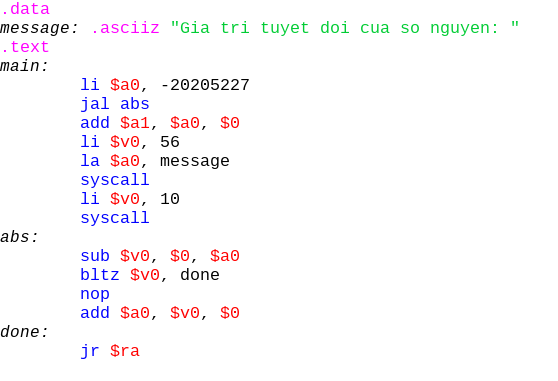
\includegraphics[width=1\textwidth]{ass1/code.png}}}
	\caption{Code của Assignment 1}
	\label{fig:ass1}
	\noindent
\end{figure}
\noindent
\textbf{Giải thích: }Đây là chương trình trả về giá trị tuyệt đối số đầu vào
\begin{itemize}
	\item Giá trị đầu vào được lưu vào \$a0.
	\item Nhảy đến hàm abs, lưu địa chỉ của câu lệnh ngay dưới vào \$ra.
	\item Thực hiện lấy 0 - giá trị \$a0 lưu vào \$v0. So sánh nếu \$v0 < 0 thì giữ nguyên giá trị \$a0, ngược lại lưu giá trị \$a0 là giá trị \$v0 hiện thời.
\end{itemize}
\clearpage
\begin{figure}[t!]
	\centerline{\fbox{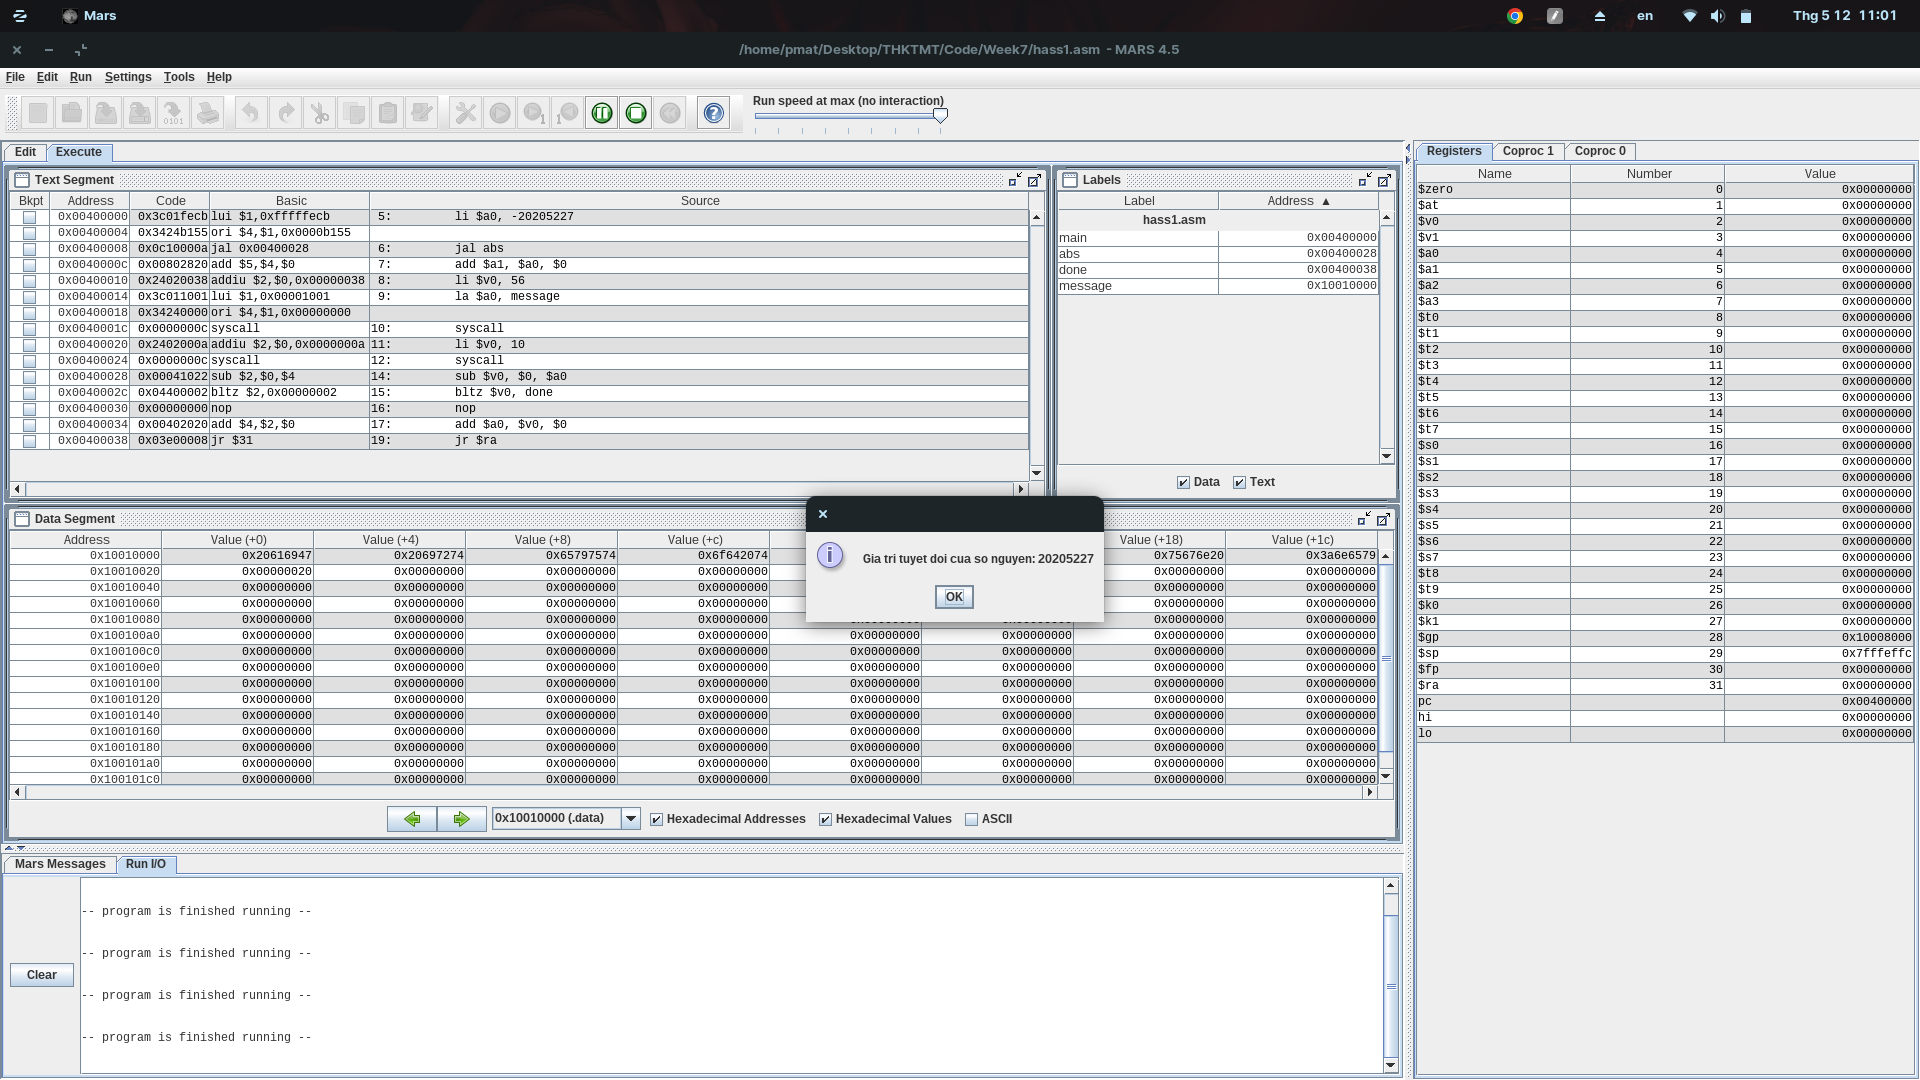
\includegraphics[width=1\textwidth]{ass1/kq.png}}}
	\caption{Kết quả của Assignment 1}
	\label{fig:ass1_kq}
	\noindent
\end{figure}
\clearpage
\section{Assignment 2}
\begin{figure}[!h]
	\centerline{\fbox{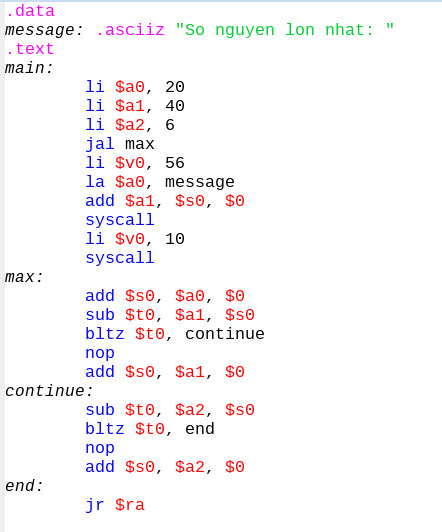
\includegraphics[width=0.9\textwidth]{ass2/code.png}}}
	\caption{Code của Assignment 2}
	\label{fig:ass2}
	\noindent
\end{figure}
\noindent
\textbf{Giải thích: }Đây là chương trình trả về số nguyên lớn nhất trong 3 đầu vào
\begin{itemize}
	\item Giá trị đầu vào được lưu vào \$a0, \$a1, \$a2.
	\item Nhảy đến hàm max, giá trị lớn nhất được lưu vào thanh ghi \$s0. Khởi tạo giá trị đầu của \$s0 = \$a0.
	\item Tiến hành so sáng \$a1 với \$s0. Nếu \$a1 > \$s0 thì tiến hành gán \$s0 = \$a1, ngược lại vẫn giữ nguyên giá trị \$s0. Tiếp tục nhảy đến hàm continue để so sánh \$s0 và \$a2. 
	\item Sau khi chạy đến hàm end. Chương trình quay về địa chỉ ngay sau lần nhảy đầu tiên (jal max) để in ra số lớn nhất ra màn hình.
\end{itemize}
\begin{figure}[!h]
	\centerline{\fbox{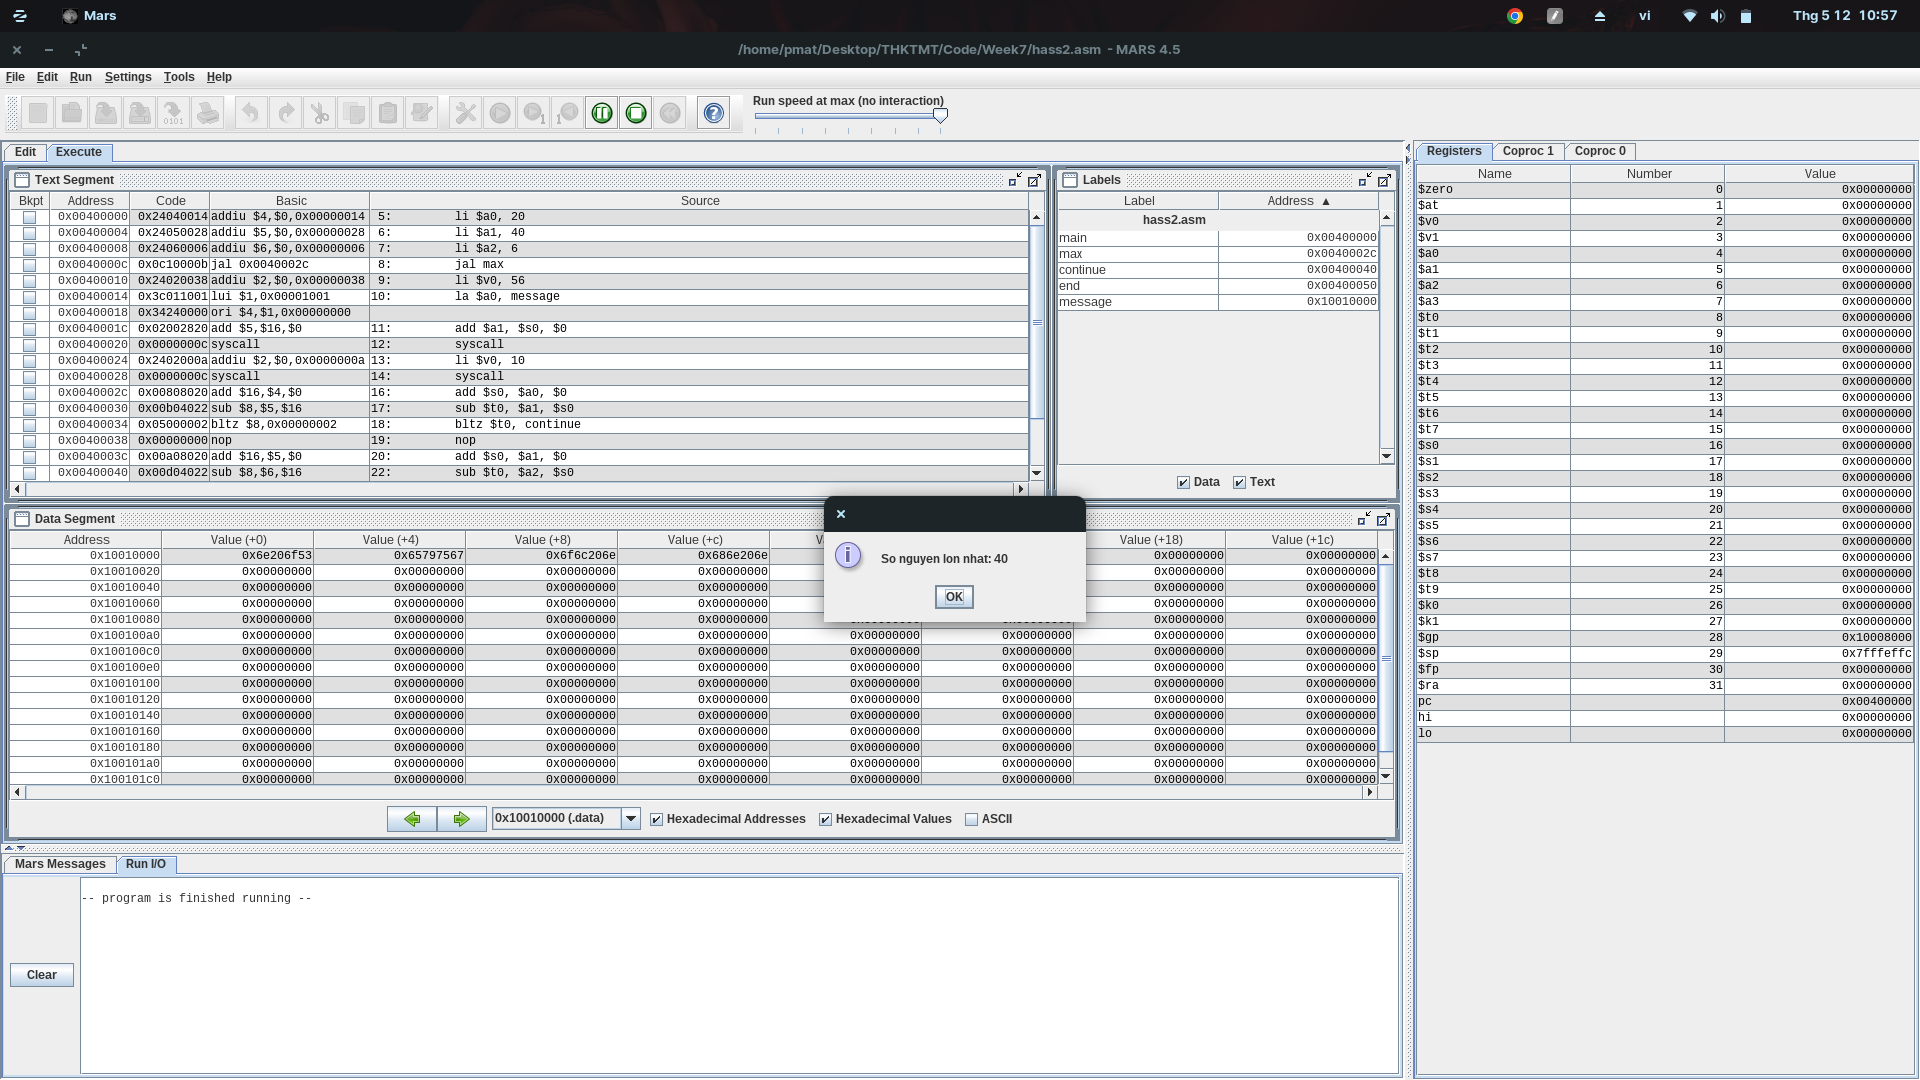
\includegraphics[width=1\textwidth]{ass2/kq.png}}}
	\caption{Kết quả của Assignment 2}
	\label{fig:ass2_kq}
\end{figure}
\clearpage
\section{Assignment 3}
\begin{figure}[!h]
	\centerline{\fbox{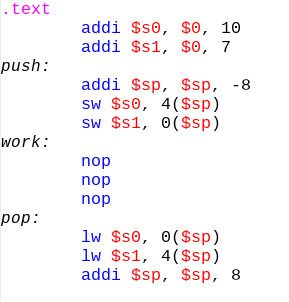
\includegraphics[width=0.7\textwidth]{ass3/code.png}}}
	\caption{Code của Assignment 3}
	\label{fig:ass3}
\end{figure}
\noindent
\textbf{Giải thích: }Chương trình swap giá trị của \$s0 \$s1 bằng stack.
\begin{itemize}
	\item Giảm nội dung của con trỏ ngăn xếp xuống 8 để lưu thêm 2 phần tử. Sau đó lưu giá trị \$s0 và \$s1 vào ngăn xếp.
	\item Load lại giá trị của \$s0 và \$s1 từ ngăn xếp. 
\end{itemize}
\begin{figure}[!h]
	\centerline{\fbox{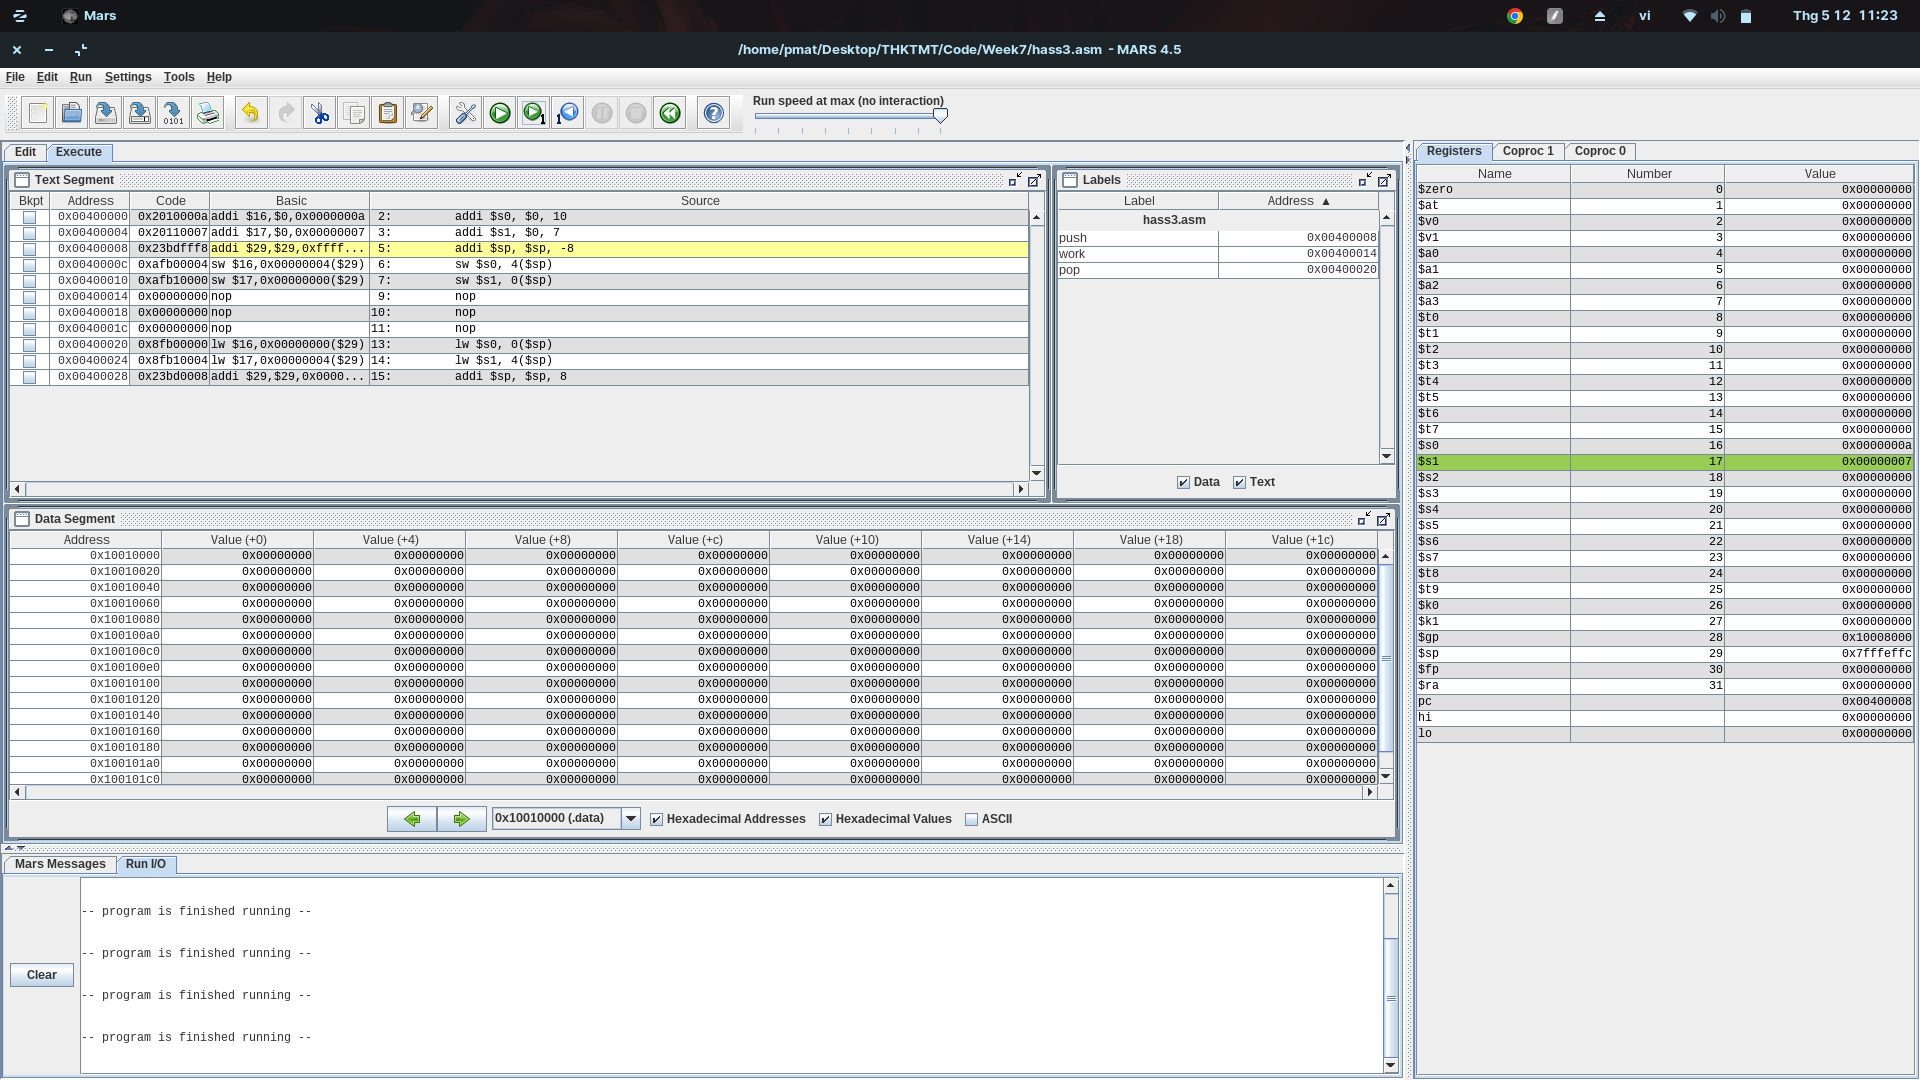
\includegraphics[width=0.8\textwidth]{ass3/1.png}}}
	\caption*{Step 1: Con trỏ \$sp đang có giá trị 0x7fffeffc}
	\label{fig:ass3_1}
\end{figure}
\begin{figure}[!h]
	\centerline{\fbox{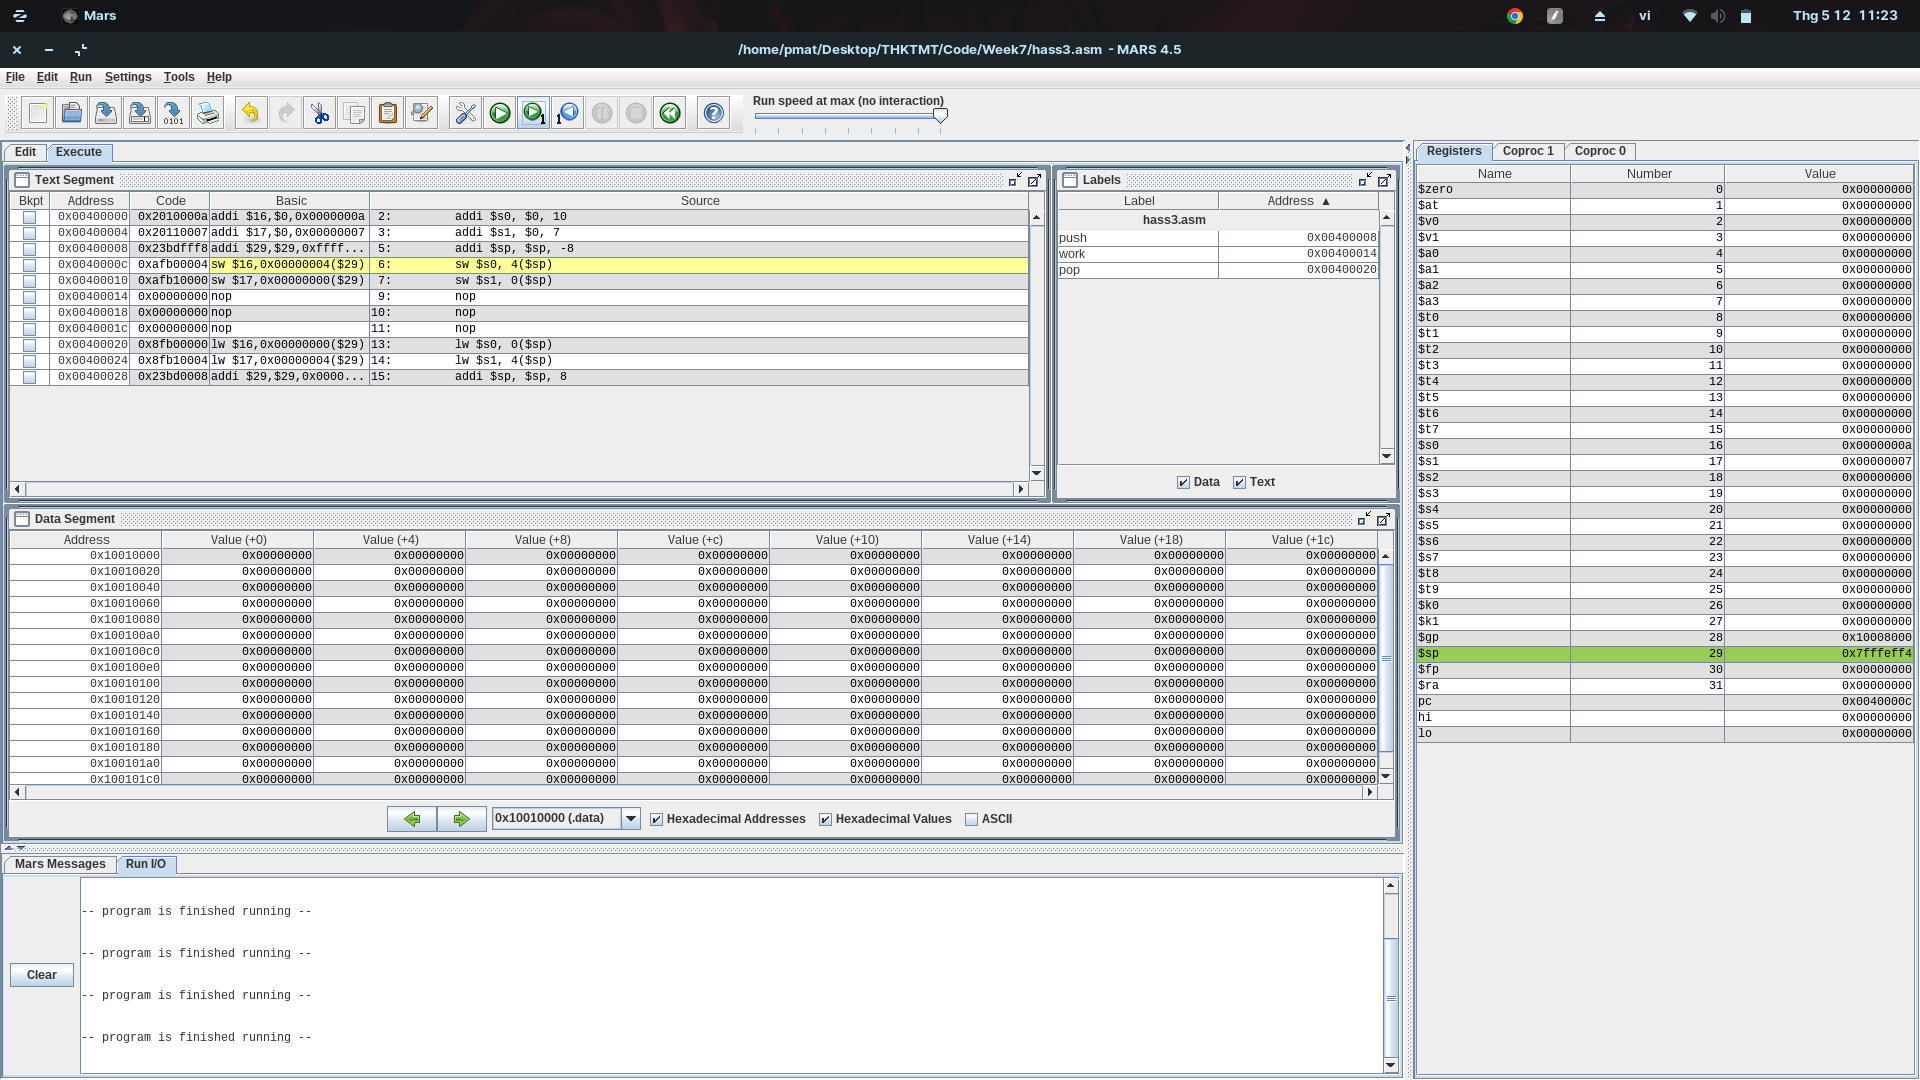
\includegraphics[width=0.8\textwidth]{ass3/2.png}}}
	\caption*{Step 2: Con trỏ \$sp chuyển thành giá trị 0x7fffeff4}
	\label{fig:ass3_2}
\end{figure}
\begin{figure}[!h]
	\centerline{\fbox{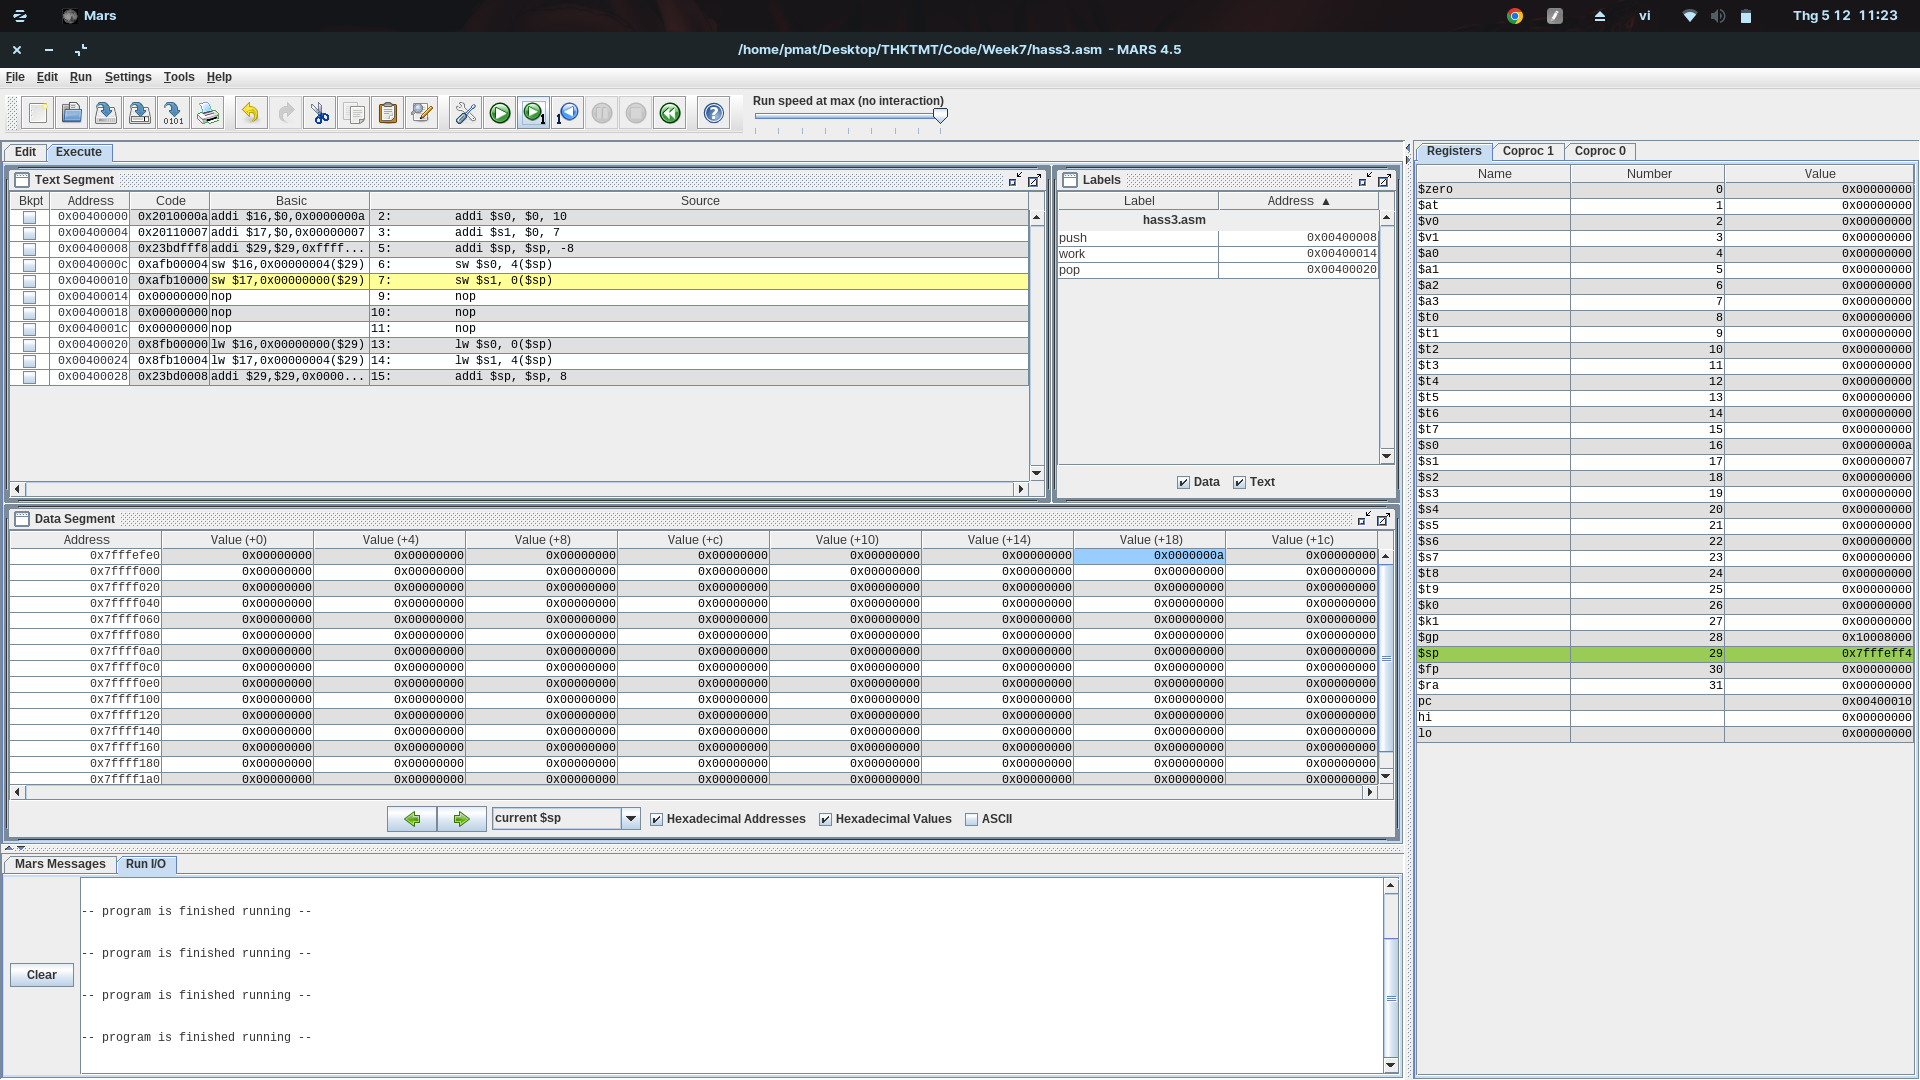
\includegraphics[width=0.8\textwidth]{ass3/3.png}}}
	\caption*{Step 3: Lưu giá trị \$s0 vào ngăn xếp}
	\label{fig:ass3_3}
\end{figure}
\begin{figure}[!h]
	\centerline{\fbox{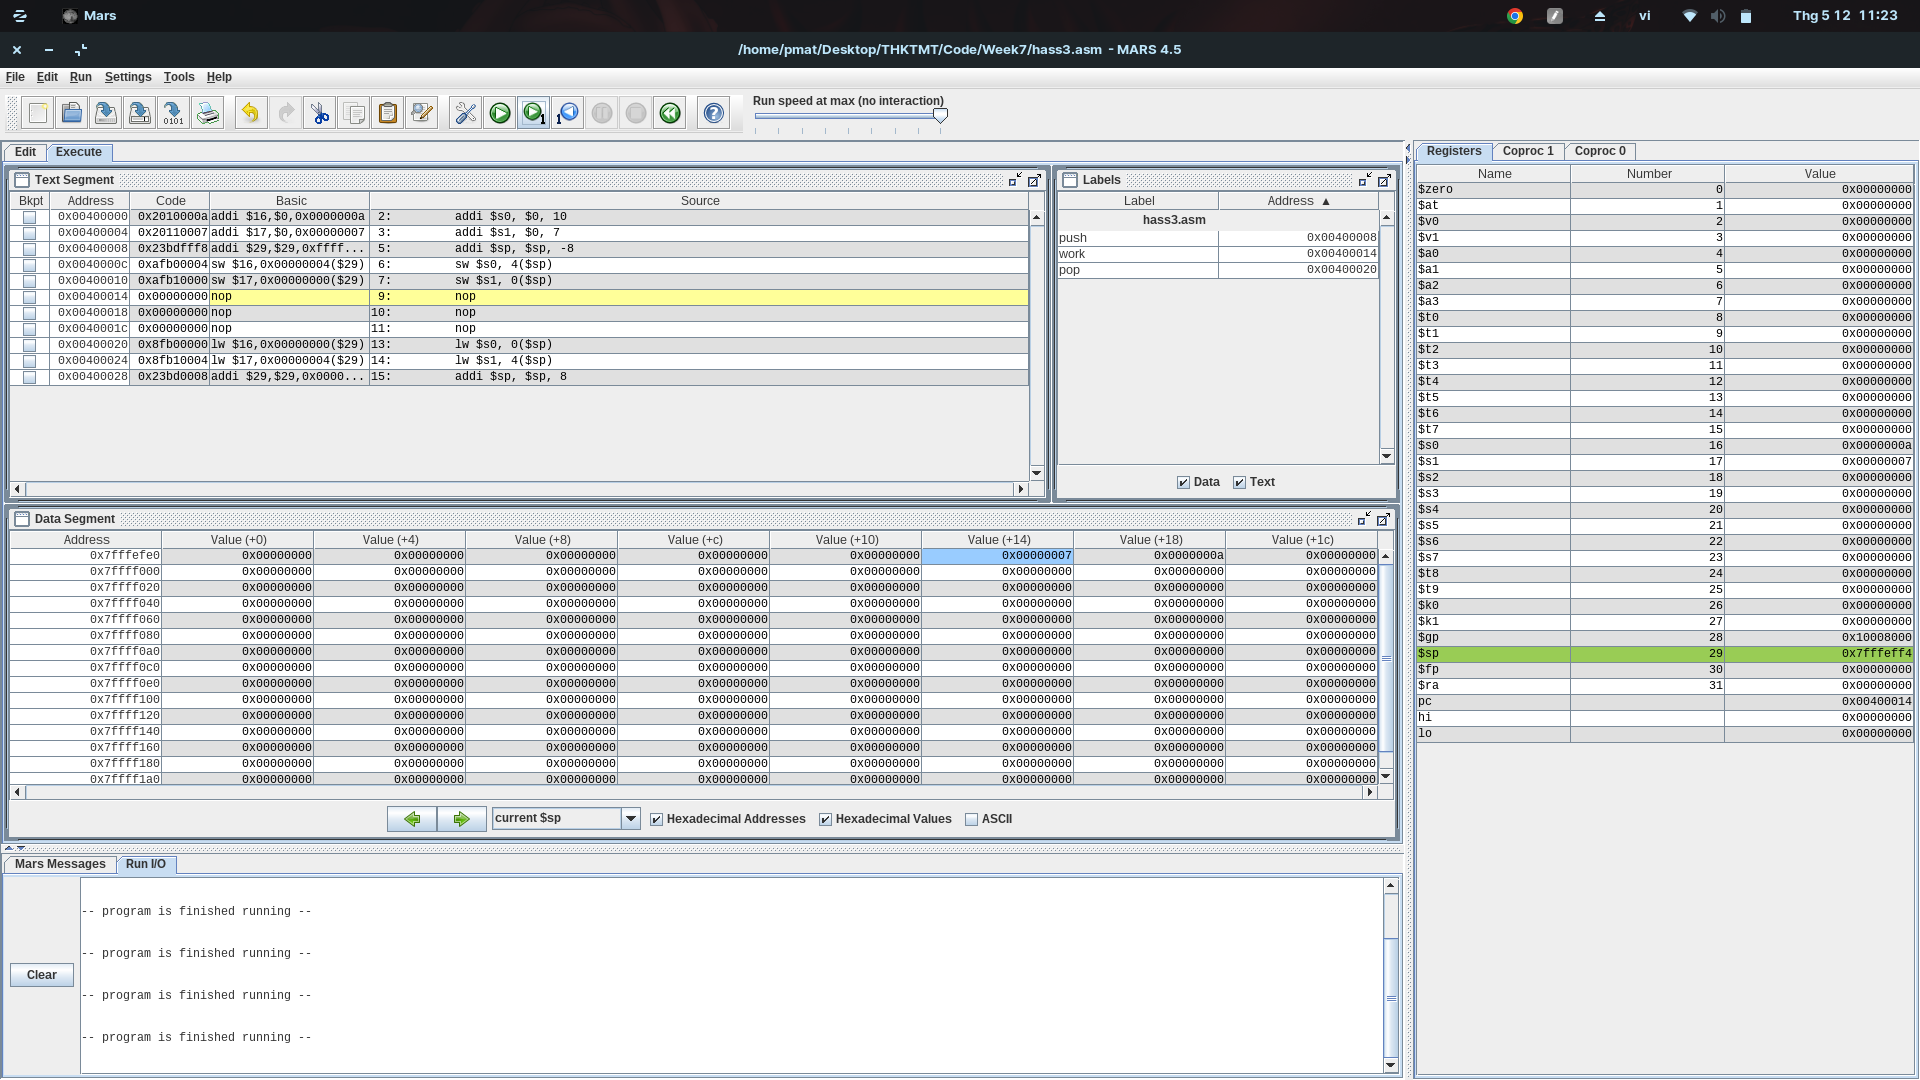
\includegraphics[width=0.8\textwidth]{ass3/4.png}}}
	\caption*{Step 4: Lưu giá trị \$s1 vào ngăn xếp}
	\label{fig:ass3_4}
\end{figure}
\begin{figure}[!h]
	\centerline{\fbox{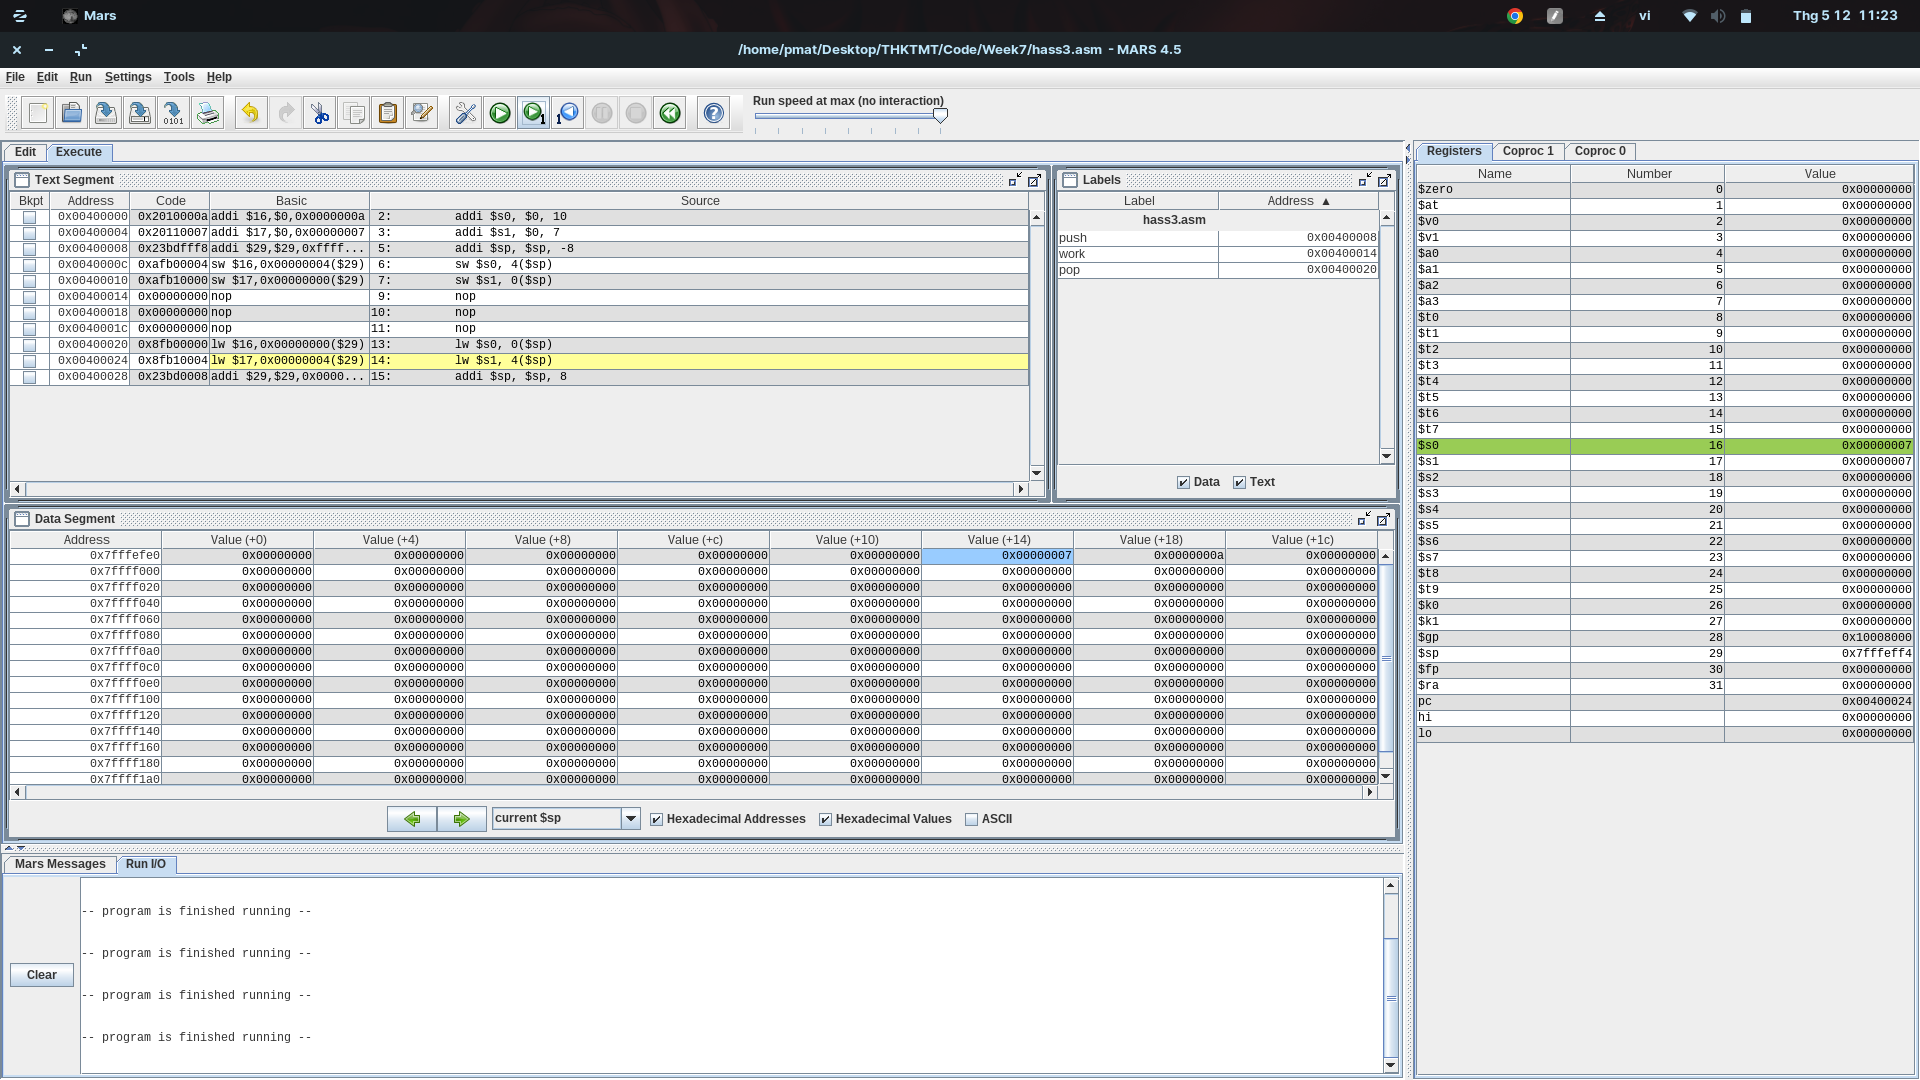
\includegraphics[width=0.8\textwidth]{ass3/5.png}}}
	\caption*{Step 5: Load giá trị \$s0 từ ngăn xếp}
	\label{fig:ass3_5}
\end{figure}
\begin{figure}[!h]
	\centerline{\fbox{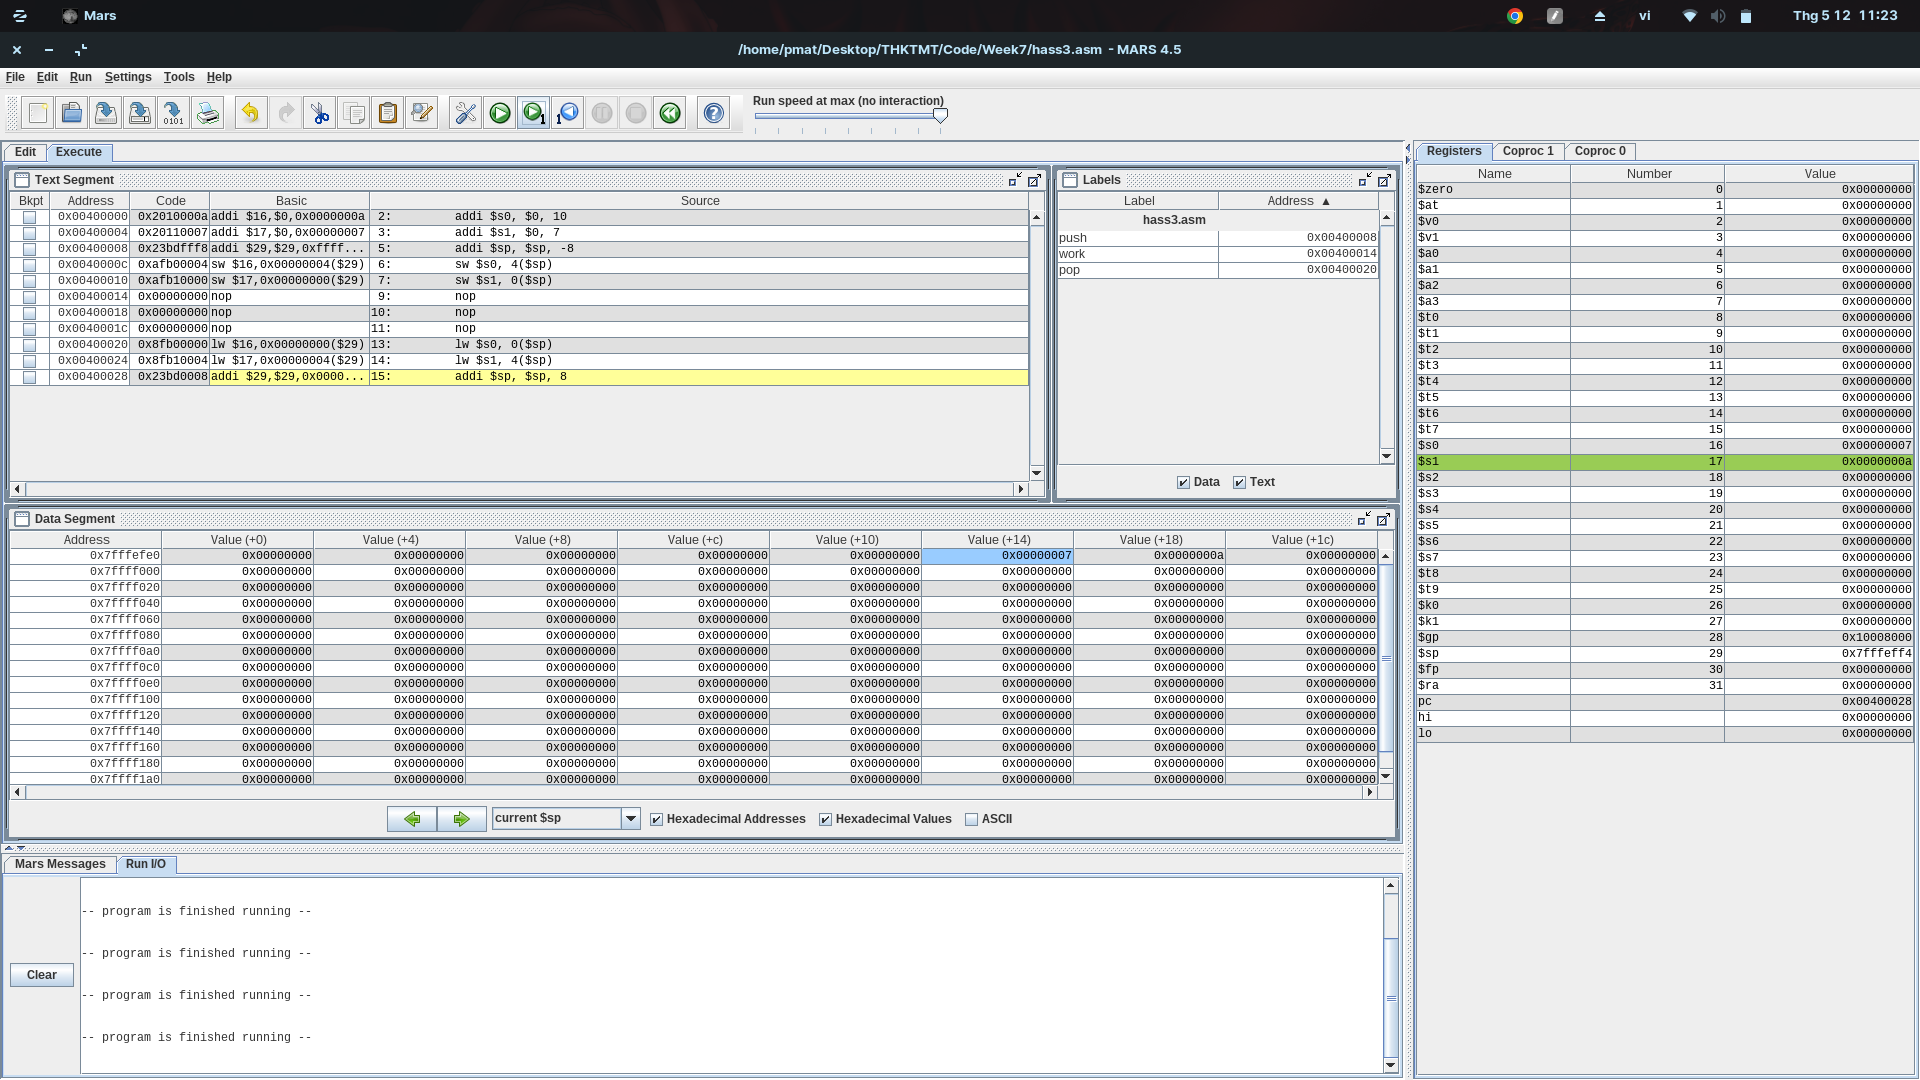
\includegraphics[width=0.8\textwidth]{ass3/6.png}}}
	\caption*{Step 6: Load giá trị \$s1 từ ngăn xếp}
	\label{fig:ass3_6}
\end{figure}
\clearpage
\section{Assignment 4}
\begin{figure}[!h]
	\centerline{\fbox{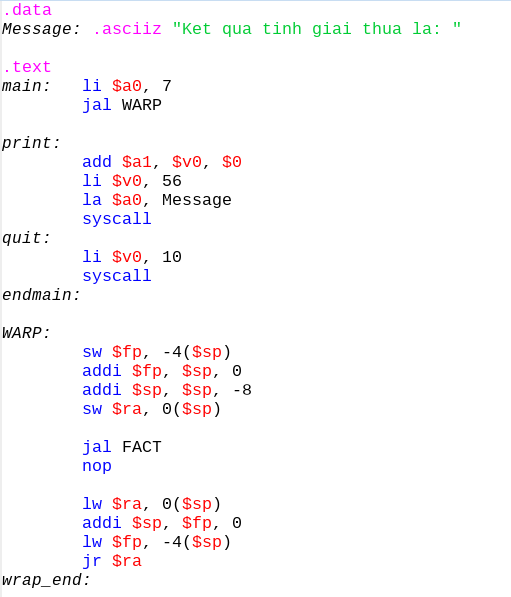
\includegraphics[width=0.5\textwidth]{ass4/code1.png}}}
\end{figure}
\begin{figure}[!h]
	\centerline{\fbox{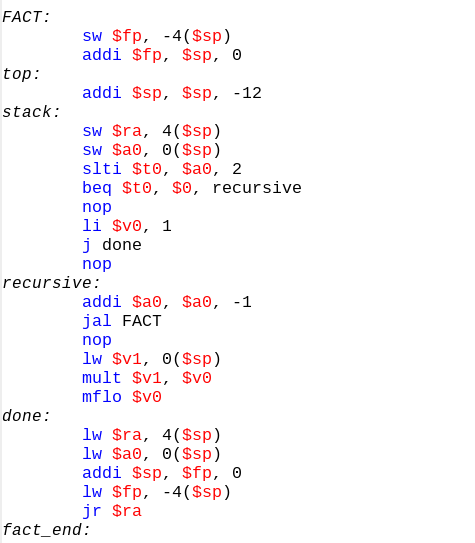
\includegraphics[width=0.5\textwidth]{ass4/code2.png}}}
	\caption{Code của Assignment 4}
\end{figure}
\clearpage
\noindent
\textbf{Giải thích:} Chương trình trả về kết quả của (\$a0)! Đoạn code dưới đây tương ứng với \$a0 = 7. \\
\textbf{Ý tưởng:} Lưu \$a0, \$fp vào stack sau đó giảm giá trị \$a0 = \$a0 - 1. Khi \$a0 < 2 thì dừng quá trình lặp, chuyển sang bước lấy giá trị từ stack để nhân vào \$v0.
\begin{figure}[!h]
	\centerline{\fbox{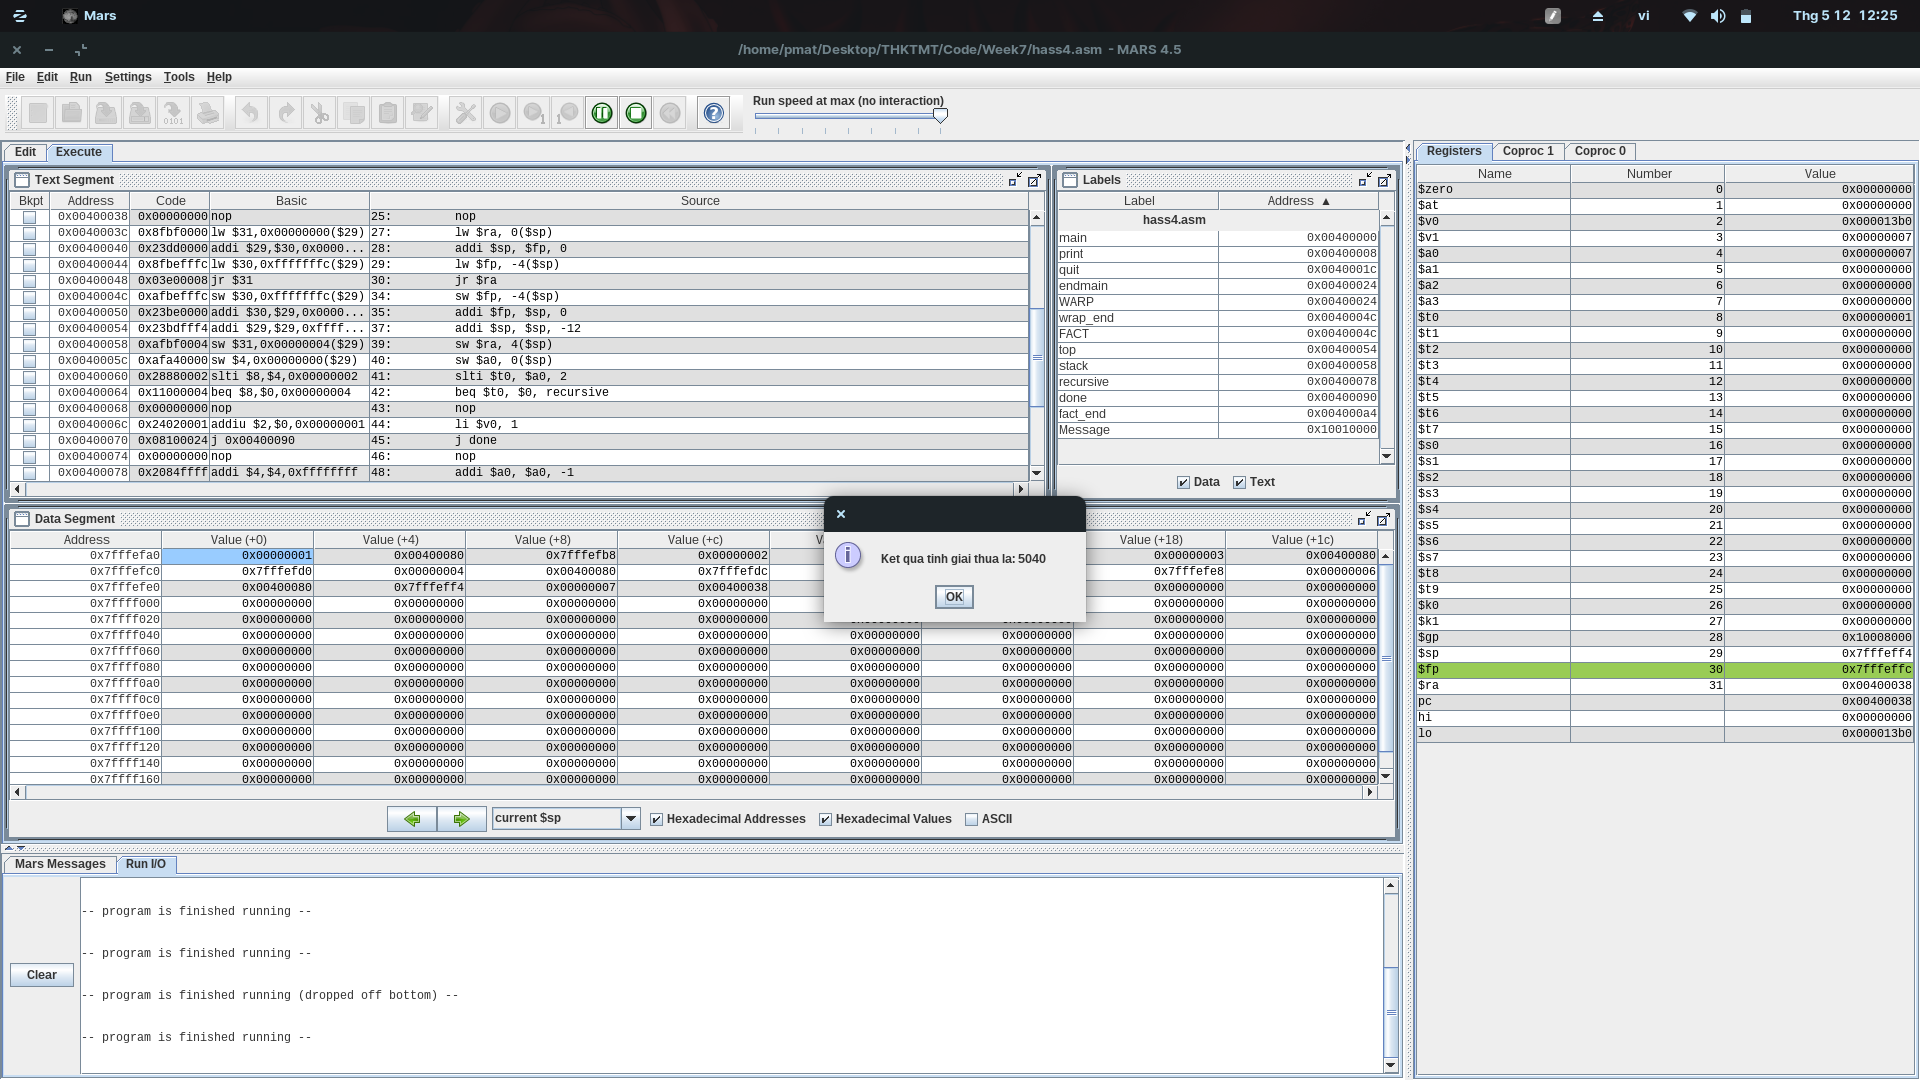
\includegraphics[width=1\textwidth]{ass4/kq.png}}}
	\caption{Kết quả của Assignment 4}
	\label{fig:ass4_kq}
\end{figure}
\begin{figure}[!h]
	\centerline{\fbox{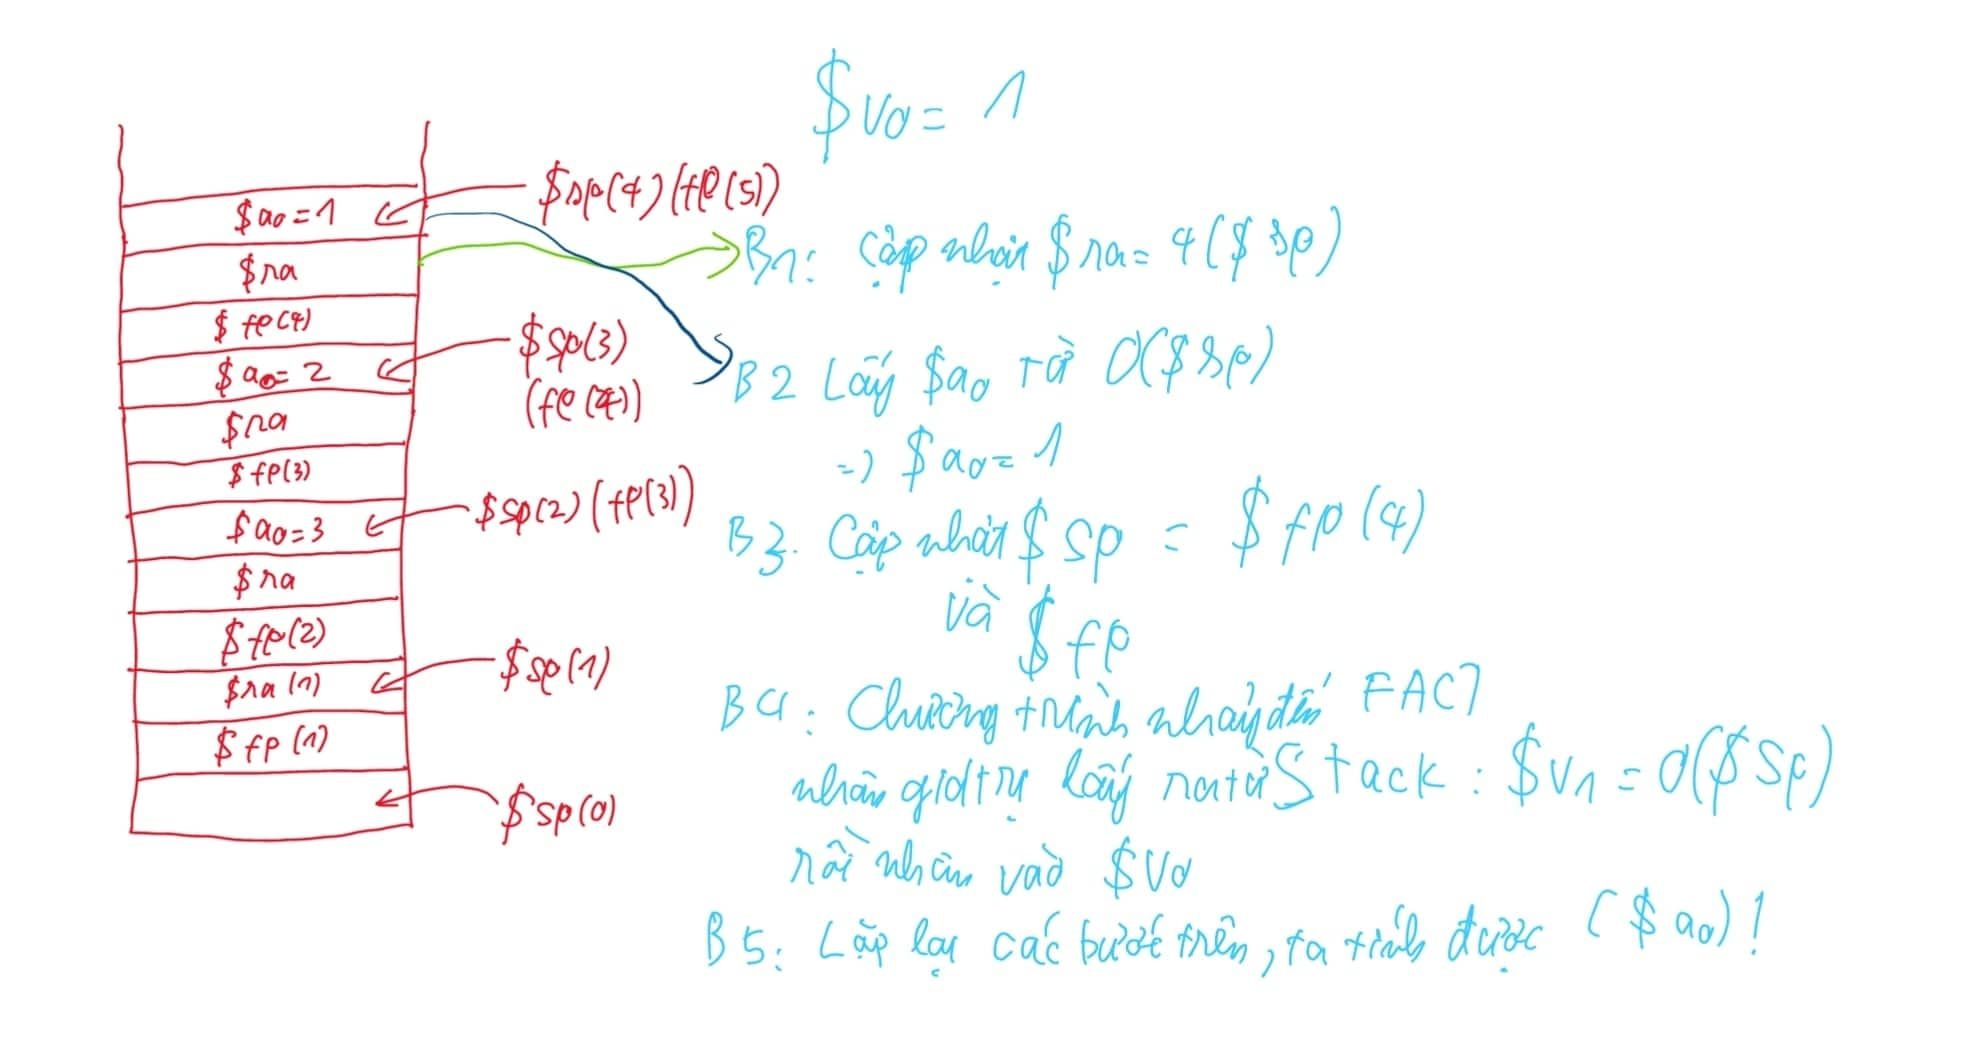
\includegraphics[width=0.9\textwidth]{ass4/tmp.jpg}}}
	\caption{Minh họa với trường hợp n = 3}
	\label{fig:ass4_kqq}
\end{figure}
\section{Assignment 5}
\begin{figure}[!h]
	\centerline{\fbox{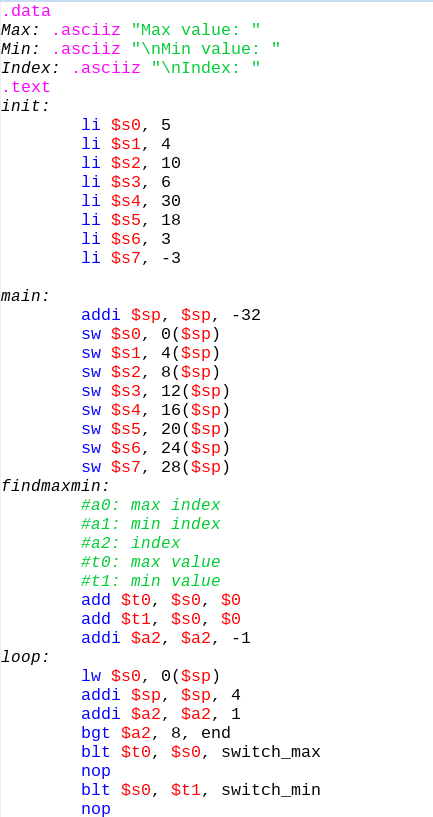
\includegraphics[width=0.5\textwidth]{ass5/code1.png}}}
\end{figure}
\begin{figure}[!h]
	\centerline{\fbox{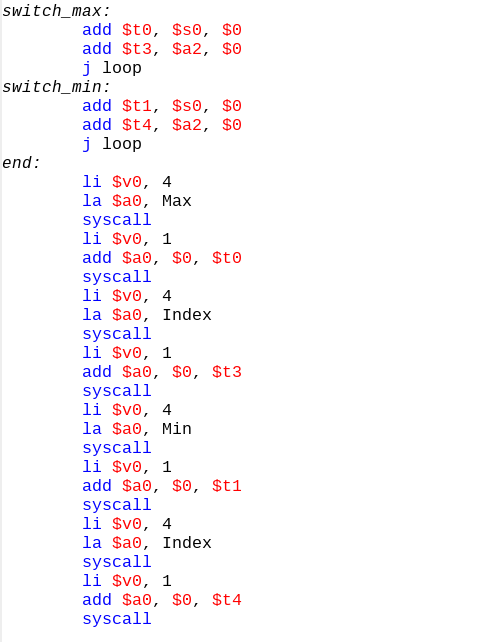
\includegraphics[width=0.5\textwidth]{ass5/code2.png}}}
	\caption{Code của Assignment 5}
\end{figure}
\textbf{Ý tưởng: }Đem các số vào trong stack, tạo 4 biến để lưu trữ giá trị lớn nhất, giá trị nhỏ nhất và index của chúng. Khi push ra từ stack ta sẽ tiến hành so sánh với các giá trị nhỏ nhất và lớn nhất hiện thời để cập nhật.
\begin{figure}[!h]
	\centerline{\fbox{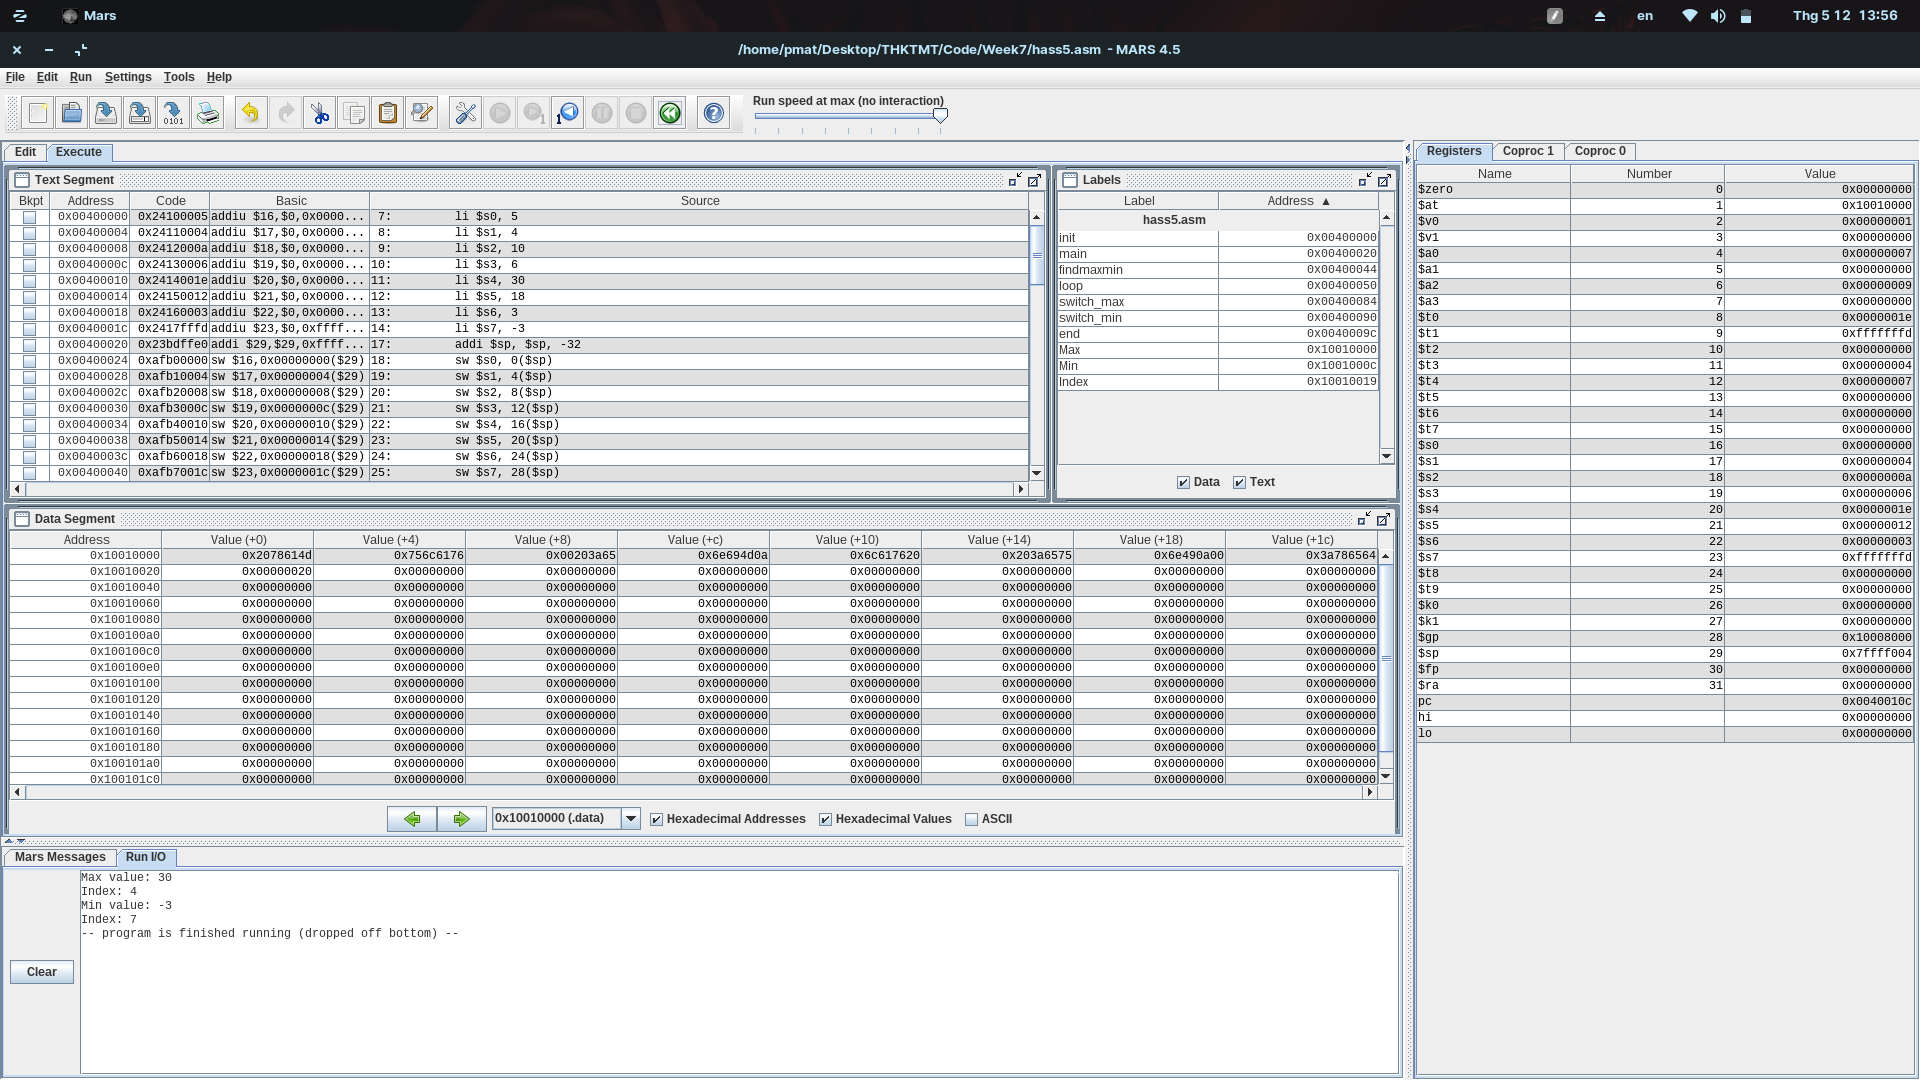
\includegraphics[width=1\textwidth]{ass5/kq.png}}}
	\caption{Kết quả của Assignment 5}
	\label{fig:ass5_kq}
\end{figure}
\end{document}